\documentclass[11pt]{article}
\usepackage[left=2cm, right=2cm, top=2cm, bottom=2cm]{geometry}
\usepackage[colorlinks=true]{hyperref}
\usepackage{amsmath}
\usepackage{graphicx}
\usepackage{float}
\begin{document}
\title{\vspace{-2em}CS145 Midterm Report\vspace{-2em}}
\date{February 18th, 2019\vspace{-2em}}
\author{}
\maketitle

\section{Team Information}

\begin{itemize}
    \item Group Number: 4
    \item Group Name: Combination Pizza Hut and Taco Bell
    \item Members: Alexander Chen, Danny Nguyen, Michael Wu, Jennie Zheng, Yijing Zhou
\end{itemize}

\section{Problem Definition and Formalization}

Companies like IMDb, Netflix, and MovieLens all include a recommendation system where users
can find potential movies given their previous browsing history and ratings. They are able
to construct user profiles with this information, and further improve the films that they
would recommend.

In this project, we are given a dataset consisting of several CSV files that include movie
metadata, user ratings, and movie genome tags. Using all of this information,
we want to evaluate several different models so that we can answer the following question:
given an unseen \{user, movie\} pair, what would the user rate that movie?

\section{Proposed Methods}

\subsection{Subtasks and Problem Formalization}

We will break this project into the subtasks of data processing, learning method implementation, and model tuning.
In the data processing stage we will try to gather our data into a format that we can easily work with. Currently
our data exists in multiple CSV files that need to be transformed into a feature vector. Then we can use this feature
vector to learn and predict ratings. We will try different learning algorithms and test and tune the hyperparameters
for these algorithms.

\subsection{Data Preparation}

Our rating data exists in tuples that contain a user ID, a movie ID, and a rating. The ID numbers do not tell us
anything about the properties of a user or movie, so we need some way to convert these into meaningful features.
We have a file that links the movie ID to a genome tag vector, which is a feature vector with the length of 1128. Each
attribute in the vector has a value from 0 to 1. One idea we have is to use this genome information as the feature
vector for the movie ID. For the user ID, we can calculate another feature vector with the same dimensionality as the
movie feature vector. We will do this by using the user's rating for a movie to weight the movie's genome tag vector
and summing across all the movies that a user has rated. This generates a user genome tag vector that indicates which types
of movies appeal to that user. Then for each movie and user pair, we can generate a similarity value by
calculating the distance between the user feature vector and the movie feature vector. We can try this using an euclidean
distance function or by taking the dot product of the two feature vectors. Then we can then train our models from this
similarity value.

Another idea that we have is to use the movie's genre information and manually generate attributes to learn from. We
can encode the genres with 1 or 0 to indicate whether a movie is categorized as a given genre or not. We could also
use other information such as the movie's release year and average movie rating. This would result in a smaller
feature vector which we would be able to more easily work with. We could also capture details that would be left
out with the genome tag approach. We would generate a user feature vector in the same fashion. This could include
attributes such as a user's average rating for movies of each genre and the total number of a user's reviews.
We will try to normalize this data and test if this produces better results.

\subsection{Learning Algorithms}

We plan to use linear regression and deep neural networks in order to learn from the data. For linear regression,
we would use gradient descent to minimize our error. We would also try to see if regularization improves
our regression. Testing must be done in order to find which regularization constant fits the best. In our deep neural
network we will use backpropagation to decrease our training error. We could tune the number of hidden layers, the
size of our hidden layers, the connectedness of our network, and the activation functions that each neuron uses.
We will submit our best model out of both of these two methods.

\section{Experiment Design and Evaluation}

\subsection{Evaluation Metric}

To assess our model's accuracy, we will use the root mean square error (RMSE) shown below.
\[\text{Error}=\sqrt{\frac{1}{n}\left(\sum_{i=1}^N \left({y_i}_\text{predicted}-{y_i}_\text{actual}\right)^2\right)}\]
This is an appropriate cost metric, because we want to minimize the difference between our predicted
ratings and the actual values. Furthermore, we want to more severely punish larger errors as opposed
to smaller errors, and thus squaring makes sense.

\subsection{Model Selection}

In order to perform model selection for different methods, we evaluate our models based upon our validation set.
We first partition our given data into mutually exclusive sets: (1) training data, and (2) validation data.
We will try to train models using linear regression and deep neural networks on the training data.
In the process we will fine-tune the hyperparameters of each method by selecting different activation functions,
changing the size of our neural networks, modifying the regularization constant, etc. Then we can select the best
model by selecting the one that achieves the lowest RMSE.

\subsection{Current Kaggle Submission}

Our current Kaggle score is 1.03952. This score was achieved simply by finding the average rating for
all the user-movie pairs in the training data and predicting that average rating for all the points in the
test data. The main purpose of trying this method was to get more familiar with the data formatting for the
Kaggle submission. It gave a surprisingly good score, beating many other teams despite the model’s simplicity.

\section{Discussion}

From the data preprocessing stage, we gained insights about the general distribution of the data. The data is right skewed
which led us to consider whether we should normalize data and which normalization methods we should choose.

\begin{figure}[H]
    \begin{center}
        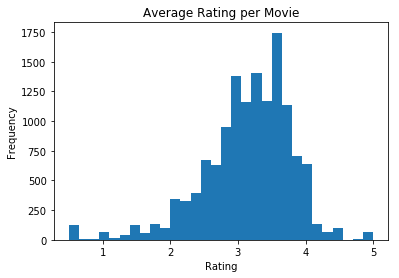
\includegraphics[width=2.5in]{AverageRatingByMovie.png}
        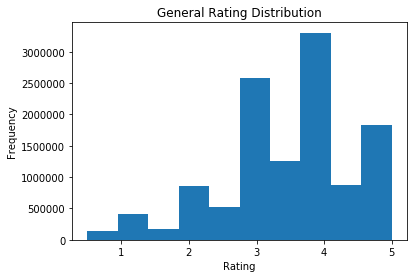
\includegraphics[width=2.5in]{RatingHistogram.png}
    \end{center}
\end{figure}

As shown in plots above, the average rating per movie is between three and four. Also, users tend to give
full rather than half scores, and there are fewer low ratings when compared to medium and high ratings.

Following those observations, we have decided to normalize the ratings so that the low scores can reflect the correct amount of
negativity. Furthermore, we have discussed whether we should round our predictions to the nearest half
or whole number. Since RMSE is used for evaluating our Kaggle submission, we have decided to keep the real values from the
predicted output. This way the performance of our models more accurately corresponds to our submission score.

Lastly, we found that there are some potential performance issue when training our models. Due to the sheer size of the data,
when we attempted to use \texttt{genome\_tags.csv} to convert the movie and user ids into feature vectors, the amount of data
caused us to run out of memory. We had to use lazy loading and other workarounds to fix the problem. We resolved the issue
by exporting our intermediate processed data as a CSV file.

\section{Schedule}

\begin{itemize}
    \item February 24th: Finish data preprocessing
    \item March 3rd: Train 2 different models: Linear Regression and Deep Neural Network
    \item March 6th: Tune hyperparameters and finalize features used
    \item March 10th: Begin final report
    \item March 16th: Double check our current Kaggle ranking
    \item March 17th: Finalize report and Kaggle submission
\end{itemize}

\section{References}

\begin{enumerate}
    \item Emmanuel, O. (2018, March). Day 1: Building a Recommendation System Using Machine Learning (ML) and Artificial Intelligence.\\
    \scriptsize
    \href{https://medium.com/the-happiness-of-pursuit/day-1-building-a-recommendation-system-using-machine-learning-ml-and-artificial-intelligence-c8b2c5ef53a8}
    {https://medium.com/the-happiness-of-pursuit/day-1-building-a-recommendation-system-using-machine-learning-ml-and-artificial-intelligence-c8b2c5ef53a8}
    \normalsize

    \item Sarwar, B. M., Karypis, G., Konstan, J., \& Riedl, J. (2002, December). Recommender systems for large-scale e-commerce:
    Scalable neighborhood formation using clustering. In Proceedings of the fifth international conference on computer and information technology (Vol. 1, pp. 291-324).

    \item Spark, C. (2018, October). Tutorial: Practical Introduction to Recommender Systems.\\
    \scriptsize
    \href{https://blog.cambridgespark.com/tutorial-practical-introduction-to-recommender-systems-dbe22848392b}
    {https://blog.cambridgespark.com/tutorial-practical-introduction-to-recommender-systems-dbe22848392b}
    \normalsize
\end{enumerate}

\end{document}